\documentclass{ximera}

\title{Graphics}

\begin{document}
\begin{abstract}
  Embed compelling content in Ximera activities.
\end{abstract}
\maketitle

We've seen basic ways to include JPGs, PNGs, and PDFs using
\verb!\includegraphics!. However, this is not the preferred way to include
graphics. Moreover, there are considerations for positioning of the graphics.

\paragraph{Positioning graphics}

In \LaTeX\ it is common to write images in the \verb!figure! environment. We
choose not to use this because \verb!figure! `floats' the images for `optimal'
page layout. We are not concerned with page layout. When working online, the
page is essentially infinite in length. Moreover, the \textit{consumers} of the
content we create are \textit{students}. Students are also unconcerned with
awkward page layout. Students prefer to see the image exactly when it is
mentioned. With this said, we suggest wrapping all images in either a
\verb!center! environment or an (Ximera-specific) \verb!image! environment.
The environment \verb!image! centers and automatically scales the contents.  If
an author finds themselves printing to various page-sizes, \verb!image! might
be preferred. Moreover, \verb!image! can be redefined globally to act
identically to \verb!center!, but \verb!center! cannot be redefined.

If you use \verb!center!, you would write something like:
\begin{verbatim}
\begin{center}
\includegraphics[width=5cm]{missionPatch.jpg}
\end{center}
\end{verbatim}
If you use \verb!image!, you would write something like:
\begin{verbatim}
\begin{center}
\includegraphics[width=5cm]{missionPatch.jpg}
\end{center}
\end{verbatim}

The disadvantage of using \verb!\includegraphics! is that you need to handle
the paths to the images in some way. You can do this by:
\begin{description}
  \item[Editing the graphics path]
  \item[Using a global graphics folder] can be done as follows by adding
\begin{verbatim}
\graphicspath{  %% When looking for inages,
{./}            %% look here first,
{./graphics/}   %% the look for a graphics folder,
{../graphics/}  %% which may be a directory up.
}
\end{verbatim}

Explain how to use a soft link to eat-your-cake and have-it too. 
You put the images in the folder with the source, then you soft link to the graphics directory. 
This is probably the best way to do it.


\end{description}
With this said, TikZ is the preferred method for graphics because code, found
in the Ximera \LaTeX\ file, generates the image. No need to worry about
graphics paths.

\section{TikZ is the preferred method for graphics}

The preferred way to include graphics is with TikZ.
\begin{image}
  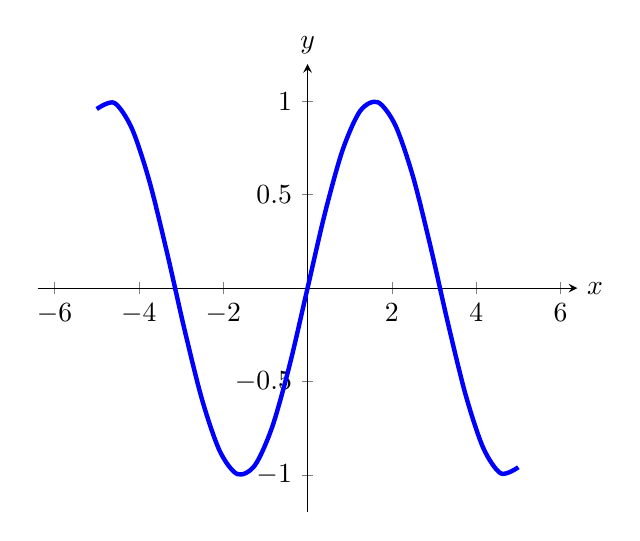
\begin{tikzpicture}
    \begin{axis}[
        xmin=-6.4,
        xmax=6.4,
        ymin=-1.2,
        ymax=1.2,
        axis lines=center,
        xlabel=$x$,
        ylabel=$y$,
        every axis y label/.style={at=(current axis.above
            origin),anchor=south},
        every axis x label/.style={at=(current axis.right of
            origin),anchor=west},
      ]
      \addplot [ultra thick, blue, smooth] {sin(deg(x))};
    \end{axis}
  \end{tikzpicture}
\end{image}

\begin{verbatim}
\begin{image}
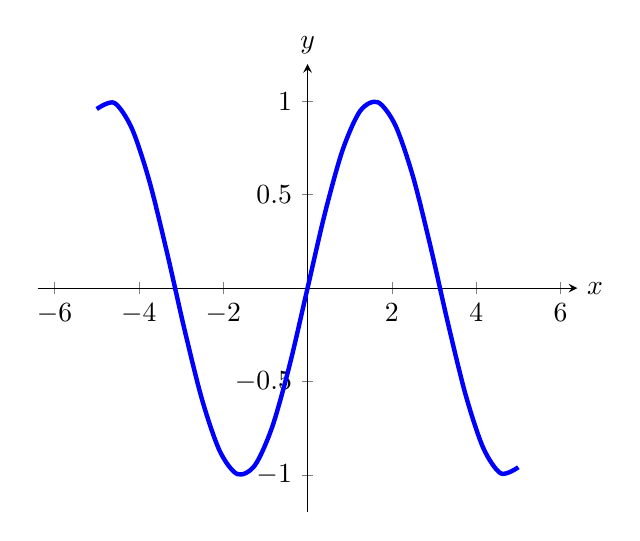
\begin{tikzpicture}
  \begin{axis}[
  xmin=-6.4,
  xmax=6.4,
  ymin=-1.2,
  ymax=1.2,
  axis lines=center,
  xlabel=$x$,
  ylabel=$y$,
  every axis y label/.style=
    {at=(current axis.above origin),anchor=south},
  every axis x label/.style=
    {at=(current axis.right of origin),anchor=west},
  ]
\addplot [ultra thick, blue, smooth] {sin(deg(x))};
\end{axis}
\end{tikzpicture}
\end{image}
\end{verbatim}


\end{document}